\section{Einarbeitung}
In der Einarbeitungsphase haben wir uns zunächst für eine Hadoop-Arbeitsumgebung entschieden. Da die meisten Projektteilnehmer über lediglich vier Gigabyte Arbeitsspeicher verfügen, fiel unsere Wahl auf die ressourcenschonende Hortonworks Sandbox\footnote{\url{http://hortonworks.com/products/hortonworks-sandbox/}}, die bei allen Teilnehmern problemlos ausgeführt werden konnte. Unter Verwendung der Sandbox haben wir den Umgang mit dem Hadoop-Ecosystem gelernt und erste Map/Reduce-Jobs ausgeführt. Darüber hinaus konnten wir weitere Tools wie Hive und Pig verwenden.

\renewcommand{\arraystretch}{1.3}

\subsection{Datenmodell}
Abbildung \ref{fig:ShoppersTables} zeigt das Datenmodell, dass aus den Entitäten "`transactions"', "`history"', "'offers"', und "`submissions"' besteht. 

\begin{figure}[H]
\centering
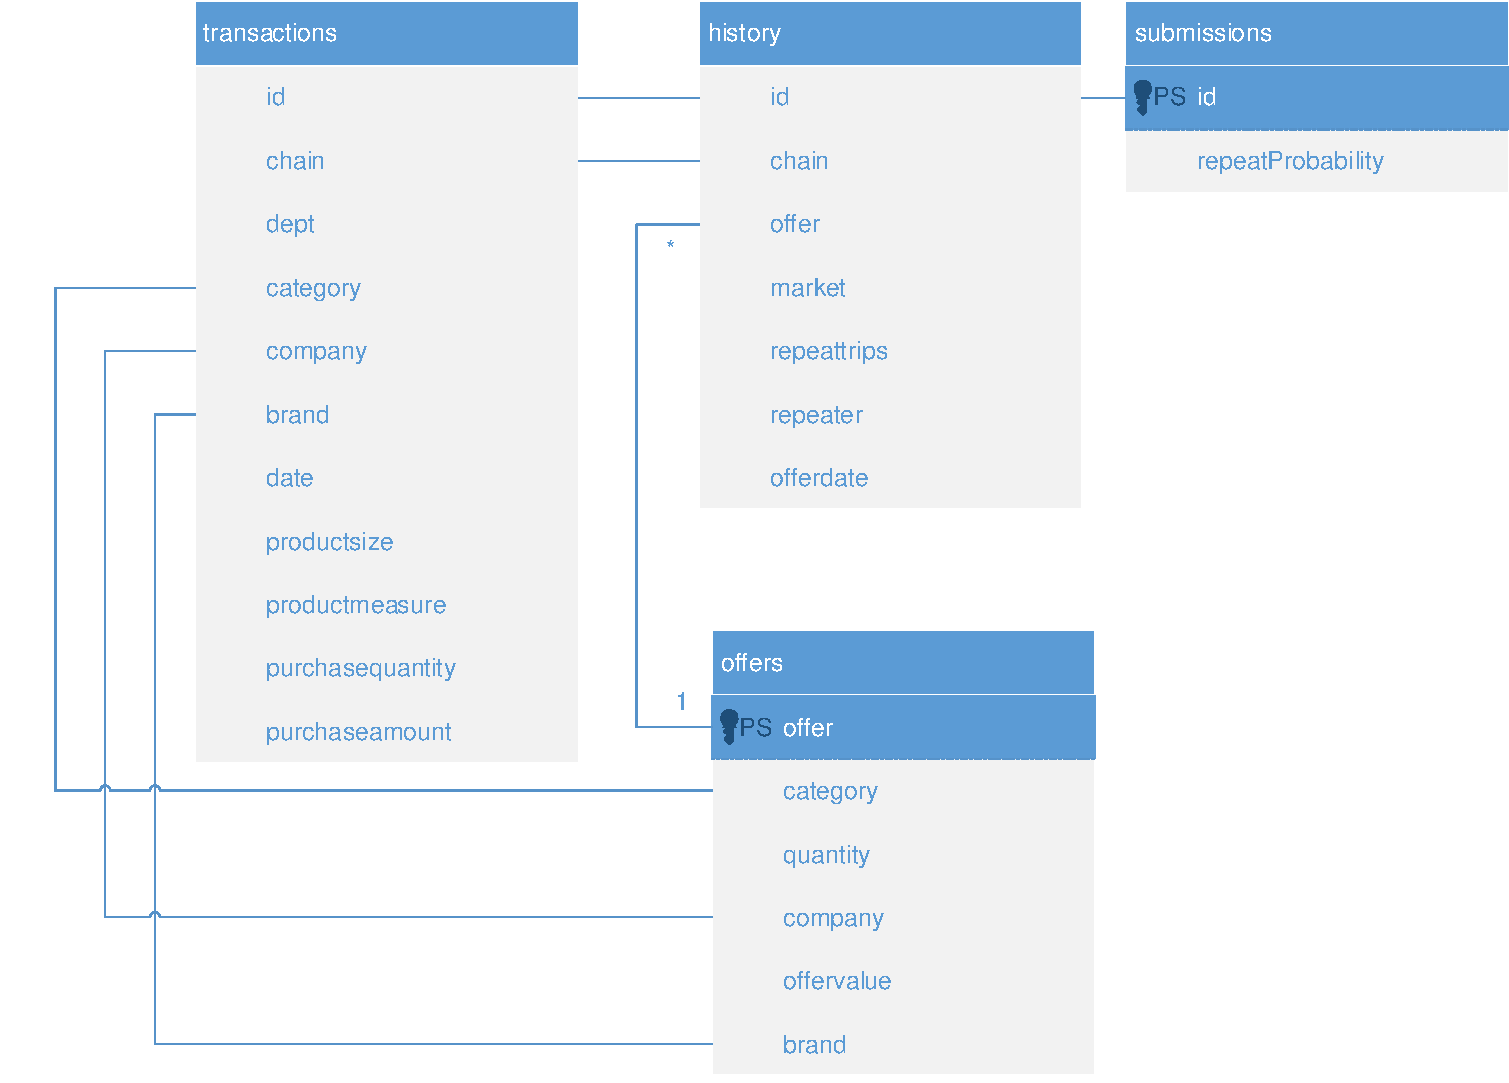
\includegraphics[width=0.93\linewidth]{Bilder/ShoppersTables}
\caption{Das Datenmodell der Shoppers-Challenge}
\label{fig:ShoppersTables}
\end{figure}

In den "`transactions"' (s. Tabelle \ref{tab:transactions}) stehen die Einkäufe der Kunden.
Die "`offers"' (s. Tabelle \ref{tab:offers}) enthalten Gutscheine, die an den Kunden verteilt wurden.
In der "`train\_history"' (s. Tabelle \ref{tab:trainhistory}) sind Informationen über die angebotenen Coupons enthalten.
Die "`test\_history"' entspricht der "`train\_history"' mit dem Unterschied, dass die beiden Felder "`repeattrips"' und "`repeater"' fehlen. Diese sind absichtlich nicht enthalten, da eine Vorhersage über diese Werte getroffen werden soll.
Die "`submissions"' (s. Tabelle \ref{tab:submissions}) enthalten die Ergebnisse, die wir bei Kaggle einreichen. Dabei wird einem Kunden eine Wiederkaufswahrscheinlichkeit zugeordnet.

Ziel dieses Projekts ist es, die Daten aus den "`transactions"', "`offers"' sowie der beiden Historiendaten zur Generierung von "`submissions"' zu nutzen. Es sollen Vorhersagen für alle Kunden-IDs aus der "`test\_history"' gemacht werden.

\begin{table}[h]
\centering
\begin{tabular}{l|l}
	 \textbf{Feld} & \textbf{Bedeutung}  \\ 
	\hline id & ID des Kunden \\ 
	\hline chain & ID der Marktkette \\ 
	\hline dept  & ID der Produktoberkategorie (z.B. Elektronikgeräte)  \\ 
	\hline category & ID der Produktkategorie (z.B. Smartphones) \\ 
	\hline company & ID der Firma die das Produkt verkauft \\ 
	\hline brand & ID der Marke (z.B. iPhone) \\ 
	\hline date & Kaufdatum \\
	\hline productsize & Menge die gekauft wurde (2L Wasser, 500g Mehl) \\ 	
	\hline productmeasure & Einheit (Liter, Gramm, Stück) \\ 	
	\hline purchasequantity & Stückzahl die gekauft wurde (Drei 2L Flaschen Wasser)
	\vspace{0.3cm} \\ 
\end{tabular}
\caption{transactions}
\label{tab:transactions}
\end{table}

\begin{table}[h]
\centering
\begin{tabular}{l|l}
	\textbf{Feld} & \textbf{Bedeutung}  \\ 
	\hline offer & ID des Coupon \\ 
	\hline category & ID der Produktkategorie \\ 
	\hline quantity & Stückzahl ab der ein Coupon gilt \\ 
	\hline company & ID der Firma die Coupons anbietet \\ 
	\hline offervalue & Preis \\ 
	\hline brand & ID der Marke
	\vspace{0.3cm} \\ 
\end{tabular}
\caption{offers}
\label{tab:offers}
\end{table}

\begin{table}[h]
\centering
\begin{tabular}{l|l}
	\textbf{Feld} & \textbf{Bedeutung}  \\ 
	\hline id & ID des Kunden \\ 
	\hline chain & ID der Marktkette \\ 
	\hline offer  & ID des Coupon  \\ 
	\hline market & ID der Region in der sich der Markt befindet  \\ 
	\hline repeattrips & Anzahl der Wiederholungskäufe (gleiches Produkt)  \\ 
	\hline repeater & Gibt an, ob repeattrips größer 0 ist \\ 
	\hline offerdate & Datum an dem der Kunde den Coupon erhalten hat 
	\vspace{0.3cm} \\ 
\end{tabular} 
\caption{train\_history}
\label{tab:trainhistory}
\end{table}

\begin{table}[h]
	\centering
\begin{tabular}{l|l}
	\textbf{Feld} & \textbf{Bedeutung}  \\ 
	\hline id & ID des Kunden \\ 
	\hline repeatProbability & Wahrscheinlichkeit das der Kunde erneut kauft 
	\vspace{0.3cm} \\
\end{tabular} 
\caption{submissions}
\label{tab:submissions}
\end{table}

\subsection{Technologieentscheidung}
Zu Beginn des Projekts haben wir uns Gedanken über die Auswahl der Technologien gemacht. Zum Zeitpunkt der Einarbeitungsphase haben wir bereits Hive und Pig durch Gruppen übergreifende Vorträge kennengelernt. Darüber hinaus standen uns keine weiteren Optionen zur Verfügung, da alternative Technologien erst zu einem späteren Zeitpunkt vorgestellt worden sind.

Somit beschränkte sich die Technologieentscheidung auf die Wahl zwischen Hive und Pig. Da wir in unserem Projekt ausschließlich Analysen auf strukturierte Daten durchgeführt haben, fiel unsere Entscheidung auf Hive. Der einfache Datenimport in Form von Tabellen und die einfachen Abfragemöglichkeiten in der SQL-ähnlichen Abfragesprache HQL waren die ausschlaggebenden Kriterien.

Die Technologien, die wir neben Hive verwendet haben, werden im weiteren Verlauf der Dokumentation erläutert.


\subsection{Data-Mining-Verfahren}
In diesem Kapitel werden wir einen Überblick über Data-Mining-Verfahren geben, die für den Einsatz im Projekt in Betracht kommen. Nach einer Erläuterung des grundlegenden Prinzips des Machine-Learning werden zwei Data-Mining-Konzepte, Regressionsanalyse und Klassifizierung, vorgestellt. Im Anschluss werden mögliche Werkzeuge zum Machine-Learning erläutert.

\subsubsection{Machine-Learning}
\label{subsubSec:MachineLearning}
Beim Machine-Learning wird versucht aus vorhanden Informationen ein Modell zu generieren, welches eingesetzt werden kann, um eine Aussage über neu hinzukommende Informationen zu treffen. Die zur Erstellung des Modells genutzten Informationen nennt man Trainingsdaten. Testdaten sind die Informationen, über die eine Aussage getroffen werden soll.

\begin{figure}[H]
\centering
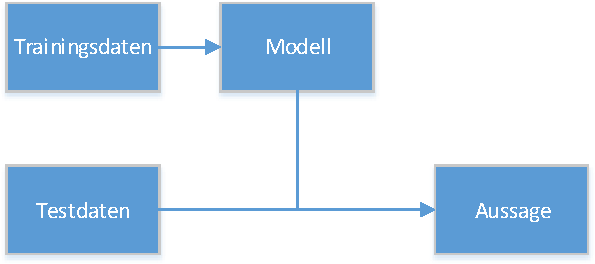
\includegraphics[width=0.7\linewidth]{Bilder/DataMining}
\caption{Machine-Learning im Modell}
\label{fig:MachineLearning}
\end{figure}

In dem Kaggle-Projekt befinden sich die Trainingsdaten in der Tabelle "`train\_history"' und die Testdaten in der Tabelle "`test\_history"'. Die Tabellen "`offers"' und "`transactions"' enthalten sowohl Trainings- als auch Testdaten. Das zu erzeugende Modell soll eine Aussage darüber treffen, ob ein Kunde erneut kaufen wird.

Das Problem lässt sich in die Kategorie des überwachten Lernens einordnen. Bei diesem werden 
einem Algorithmus Paare aus Eingabedaten und Funktionswerten übergeben. Der Algorithmus erstellt
daraus ein Modell, das zu einer neuen Eingabe eine Aussage über den Funktionswert trifft. Beispiele für
das überwachte Lernen sind Regressionsanalyse und Klassifizierung.
 
Im Rahmen dieses Projekts werden wir uns deshalb vorrangig mit dem überwachten Lernen beschäftigen. 
Denkbar sind zum einen eine Regressionsanalyse und zum anderen eine binäre Klassifizierung.
Für dieses Projekt kann man sich eine Regressionsanalyse vereinfacht so vorstellen, dass man eine Menge
von Eingabedaten hat und eine Funktion findet, die dafür einen Funktionswert zwischen 0 und 1 generiert. 
Dieser Wert stellt die Wahrscheinlichkeit dar, dass ein Kunde erneut kauft. Da der Kunde insgesamt nur 
zwei Möglichkeiten hat, kann eine binäre Klassifizierung eingesetzt werden, bei denen folgende Klassen 
unterschieden werden:

\begin{description}
	\item[0:] Der Kunde kauft nicht erneut
	\item[1:] Der Kunde kauft erneut
\end{description}
Die Klassifizierung soll eine Aussage treffen, mit welcher Wahrscheinlichkeit ein Testdatensatz zur Klasse 0 bzw. 1 gehört.

Sowohl bei der Regressionsanalyse, als auch bei der Klassifizierung gibt es das Problem der Überanpassung (auch Overfitting genannt). Von Overfitting spricht man, wenn ein Algorithmus die Trainingsdaten auswendig gelernt hat.
Die erzeugte Funktion passt damit nur auf die Trainingsdaten und kann nicht auf weitere
Testdaten verallgemeinert werden. Zur Verhinderung von Overfitting übergibt man nur die wichtigen bzw. relevanten Daten an den Algorithmus zur Erstellung des Modells. Diese Einschränkung der Daten nennt man Feature-Selection.

\subsubsection{Online- und Offline-Machine-Learning}

Beim Machine-Learning gibt es zu den vorgestellten Kategorien noch zwei Oberkategorien, zum einen das 
Online-Machine-Learning und zum anderen das Offline-Machine-Learning. 
Beim Online-Machine-Learning nimmt der Algorithmus schrittweise je einen Datensatz aus den Trainingsdaten
und passt daraufhin das Modell an.
Daher kann bei diesem Verfahren das Modell erweitert werden. 
Dies ist zum Beispiel dann von Vorteil, wenn man ein Modell über Trainingsdaten der letzten Jahre hat und dieses um die Daten der vergangenen Tage erweitern will. Der Nachteil ist allerdings, dass die Reihenfolge, in der die Trainingsdaten eingelesen werden, Einfluss auf das Modell hat.
Im Gegensatz dazu können beim Offline-Machine-Learning nur einmal Trainingsdaten übergeben werden. Diese werden unabhängig von der Reihenfolge verarbeitet. Tabelle \ref{tab:MachineLearningTrainingData}
fasst die Unterschiede der beiden Verfahren zusammen.

\begin{table}[H]
	\centering
\begin{tabular}{l|c|c} 
	\textbf{} & \textbf{Offline-Learning} & \textbf{Online-Learning}  \\  
	\hline \textbf{Reihenfolge entscheidend} & nein & ja \\
	\hline \textbf{Modell erweiterbar} & nein & ja 
	\vspace{0.3cm} 
\end{tabular} 
\caption{Trainingsdaten beim Machine-Learning}
\label{tab:MachineLearningTrainingData}
\end{table}
 
\subsubsection{Werkzeuge}
In diesem Kapitel stellen wir Werkzeuge für Machine-Learning vor, die für dieses Projekt infrage kommen.

\begin{description}
\item[Vowpal Wabbit] Vowpal Wabbit\footnote{\url{https://github.com/JohnLangford/vowpal_wabbit/wiki}} ist ein Open-Source-Programm für Online-Machine-Learning. Es wurde ursprünglich bei Yahoo! Research entwickelt und wird heute von Microsoft Research unterhalten. Es bietet die Möglichkeit Klassifizierungs- und Regressionsalgorithmen zu verwenden.

\item[Apache Mahout] Apache Mahout\footnote{\url{http://mahout.apache.org/}} ist ein Projekt zur Implementierung von Machine-Learning, das in erster Linie auf Collaborative-Filtering, Clustering und Klassifikation fokussiert ist. Die bekanntesten Implementierungen von Mahout setzen auf Hadoop auf und nutzen das Map/Reduce-Verfahren. Eine Einbindung von Mahout in AWS ist relativ einfach zu bewerkstelligen.

\item[Glmnet] Glmnet\footnote{\url{http://cran.r-project.org/web/packages/glmnet/index.html}} ist ein R-Package, das lineare und logistische Regression implementiert.
\end{description}

Die Tabelle \ref{tab:MachineLearningTools} stellt die möglichen Anwendungsumgebungen der Implementierungen dar:

\begin{table}[H]
	\centering
\begin{tabular}{l|c|c|c} 
	\textbf{} & \textbf{HDFS (HortonWorks)} & \textbf{AWS} & \textbf{Lokal}  \\  
	\hline \textbf{Vowpal Wabbit} & - & - & x \\
	\hline \textbf{Apache Mahout} & x & x & x \\
	\hline \textbf{Glmnet} & x & x & x 
	\vspace{0.3cm} 
\end{tabular} 
\caption{Anwendungsumgebungen der Machine-Learning-Werkzeuge}
\label{tab:MachineLearningTools}
\end{table}

